\chapter{Communication protocol}\label{chap:comm}
For the main hardware components to be able to communicate, some kind of network communication has to be defined. Throughout this chapter the communication hardware, methods and final design of this network will be introduced.

\nomenclature{SPI}{Serial Peripheral Interface}

\section{Low level protocol specification}
In \marginnote{Not sure about the exact placement of each part of section. Let's talk about that some day!}[-25pt] the assignment proposal it is given that the communication interface between the FPGA and LM3S6965 microcontroller must be SPI. There are no formal SPI protocol standards however, so it must be decided how the link will work. The Stellaris SSI\footnote{Synchronous Serial Interface} module supports three different interfaces: Freescale SPI, MICROWIRE and Texas Instruments SSI. The main difference between these three formats is how they handle each individual serial frame.

The Freescale SPI mode of operation is chosen, as it enables full-duplex transmission (which MICROWIRE does not) and because of the way the select signal (\texttt{SSIFss}) works in this mode. Using the Freescale frame format, the \texttt{SSIFss} is high while the communication line is idle. \marginnote{This calls for an illustration} It is then pulled low while sending a frame. Pulling it low thus signifies the beginning of a frame, and pulling it high tells the slave that the frame is at its end. The Texas Instruments SSI format works by instead pulsing its \texttt{SSIFss} signal for only one \texttt{SSIClk} period to signify the beginning and ending of a frame. This is deemed more error prone as there is no time in-between frames to synchronize. Freescale SPI has one \texttt{SSIClk} period in-between frames, where \texttt{SSIFss} gets pulled high, allowing the slave a chance to "catch up".\nomenclature{SSI}{Synchronous Serial Interface}

The LM3S6965 microcontroller will be operating as master and the FPGA as slave, letting the microcontroller when communication should take place.

%------------------------------------------
\subsection{SPI introduction}
As SPI is a commonly used transmission interface, this will only contain a short introduction. SPI is short for Serial Peripheral Interface, and is a commonly used standard for internal communication.  A the simplest SPI connection consists of a master, a slave and 4 signal lines: A clock, a signal from master to slave (MOSI\footnote{Master Out Slave In}), a signal from slave to master (MISO\footnote{Master In Slave Out}) and a slave select (SS) signal. The clock is used to control when to put data on the signal lines, and is always controlled by the master device. This way the master devices always controls when there is data available on the signal lines, and at what data rate the it is send. The synchronisation between the clock and the data on the MOSI and MISO lines can be set up in four different ways, depending on the clock phase (CPHA) and polarity (CPOL). The slave select signal is used to enable the transmission on the slave device. When pulled low, the slave device starts listening for data from the master device. This enables the use of the clock, MOSI and MISO lines for multiple device. 
% What is SPI
% Limitations

%CPOL CPHA

% SPI stands for Serial Peripheral Interface
% Used for moving data simply and quickly from one device to another
% Serial Interface
% Synchronous
% Master-Slave
% Data Exchange
% Data on SCK  (the clock rate can vary, unlike RS-232 style communications)
% SPI sync modes
% WIKI fact:  frequencies are commonly in the range of 1�70 MHz

%\subsection{Hardware support}
% Support on ARM development board -- The LM3S6965 controller includes one SSI module that provides the functionality for synchronous
% serial communications with peripheral devices, and can be configured to use the Freescale SPI,
% MICROWIRE, or TI synchronous serial interface frame formats. The size of the data frame is also
% configurable, and can be set between 4 and 16 bits, inclusive.

% Separate transmit and receive FIFOs, 16 bits wide, 8 locations deep

%\subsection{Inspiration for protocol}
% ArcNet / PA10
% CAN / DeviceNet
% ADNS9500 Mouse sensor, IMU sensor
% - What is it used for, and why is it interesting to look at?
%The first approach for designing the SPI protocol was to look for  
\subsection{Protocol requirements}
Selection the right protocol design for a project greatly depends on the requirements from the other parts as the system. Such requirements would include: 
\begin{itemize}
\item Noise on transmission lines (Need for error correction or detection)
\item Security (encryption)
\item Package synchronisation
\item The size of data to be transmitted (Minimum transmission speed)
\item Timing criteria (Do we need to know how old the data are)
\end{itemize}

Because the data only needs to travel a short distance, noise and security is not considered as a problem in this project. Even if noise should occur, a lot of things could be done to the physical parts to solve this without involving redesign of the protocol (Ex. paired and shielded cables). 
The protocol are using SPI, so there is no need for synchronising the packages, as this can be done by the SS signal line. This eliminates the needs for overhead such as start or stop flags on packages. 

SPEED REQUIREMENTS ??

Because the protocol carries important data for the control system, the timing criteria needs to be taken into consideration. Tough the actuators controlled by the control system are relatively slow compared to the transmission speed, (?? how fast does this need to be?)


\subsection{Protocol ideas}
\label{spi_protocol_ideas}
During the design of the protocol three approaches were considered. These three approaches and the final protocol solution are described below.


\subsubsection{Specialised protocol}
The first approach was to design the protocol to carry just the information that needs to be exchanged between the FPGA and ARM boards. This idea had the advantage of a low overhead on the protocol and thereby a minimal need for resources on the platforms. This idea was discarded, because a change in the data requirements would require a redesign of the protocol.

\subsubsection{Memory synchronisation protocol}
Another approach to the protocol design was to make a protocol to synchronise a static sized memory between the two platforms. The idea was to take advantage of the 16bit x 8 FIFO on the ARM platform, so one package would fit exactly into it. The advantage would be that the ARM platform only needs to be interrupted when the FIFO was full. A similar solution would then be written in hardware to the FPGA, making this solution quite efficient. The large amount of data in one package would allow a CRC or checksum to be implemented without too much overhead. An example of how this protocol could be made is shown in figure \ref{fig:spi_protocol_format_memsync}.

\begin{figure}[htb]
	\begin{center}
	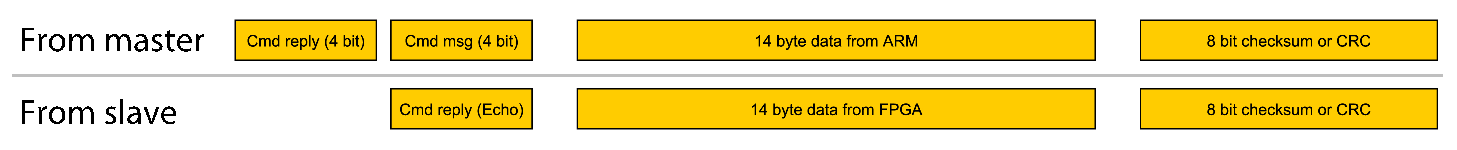
\includegraphics[scale=0.7,trim=0 380 0 380]{graphics/spi_protocol_format_memsync.pdf} %trim=l b r t (can cut off from every side)
	\caption{An example of the protocol design with the memory synchronisation protocol approach. The upper line is data from master to slave, the next is data from slave to master. The first four bits from the master decides what the slave shall respond. The next four bits describes what the master is sending to the slave. After the slave has received the first four bits, it immediately echoes the command followed by the requested data.}
	\label{fig:spi_protocol_format_memsync}			% figure labels are of the form \label{fig:*}
	\end{center}
\end{figure}


\subsubsection{Generic protocol}
The generic approach was to make the protocol compatible with the protocol of other SPI devices. This will give the great advantage of both reusable code and hardware. The generic design approach was chosen as most appropriate solution for this project and will be described in grater details in section \ref{spi_rotocol_design}.


\subsection{Protocol selection discussion}
Something that sounds smart...

%The ADNS9500 mouse sensor and ADIS16405 IMU sensor SPI interface protocols were used as reference designs, as these are well known form earlier projects.  

% Burst mode
% i2c
% error correction / detection
% Error detection
% Room for extending protocol

\subsection{Protocol design}
\label{spi_rotocol_design}
It has been decided to use a generic way of communicating between the FPGA and ARM board. Other ideas were considered and can be read about in \ref{spi_protocol_ideas}.
The main advantage for choosing a generic design is the compatibility with other SPI devices. The ADNS9500 mouse sensor and the ADIS16405 IMU sensor were used as reference devices, as these were used in previously projects. The main difference between the protocol in these two devices are the length of the carried data. The ADNS9500 reads and writes only 8 bits at a time, where ADIS16405 supports 16bit data sizes. The 8 bit solution was chosen as reference.

For synchronisation of clock and data on the signal lines, mode 0 was chosen. Mode 0 is when data is available on clock rising edge and changes on falling edge.

The general idea is that the SPI slave has a memory block, which the SPI master can read and write from. Depending on the address it can be read only, write only or read/write. The list of addresses and read/write permissions can be found in the device datasheet. The protocol itself is pretty straight forward. The MSB determines if it is a read or write operation, and the last 5 bits determines the address or function. The two bits in between are reserved for future use, and should always be set to zero. The five address bits in the current design gives access to 32 bytes of memory on the slave device, which is enough to hold the data for this project. The command structure is shown in figure \ref{fig:spi_protocol_cmd_structure}. Both reference devices supports a burst command, where a series of relevant data are sent as response of a single command. There was no need to implement such functionality in this design.
\begin{figure}[htb]
	\begin{center}
	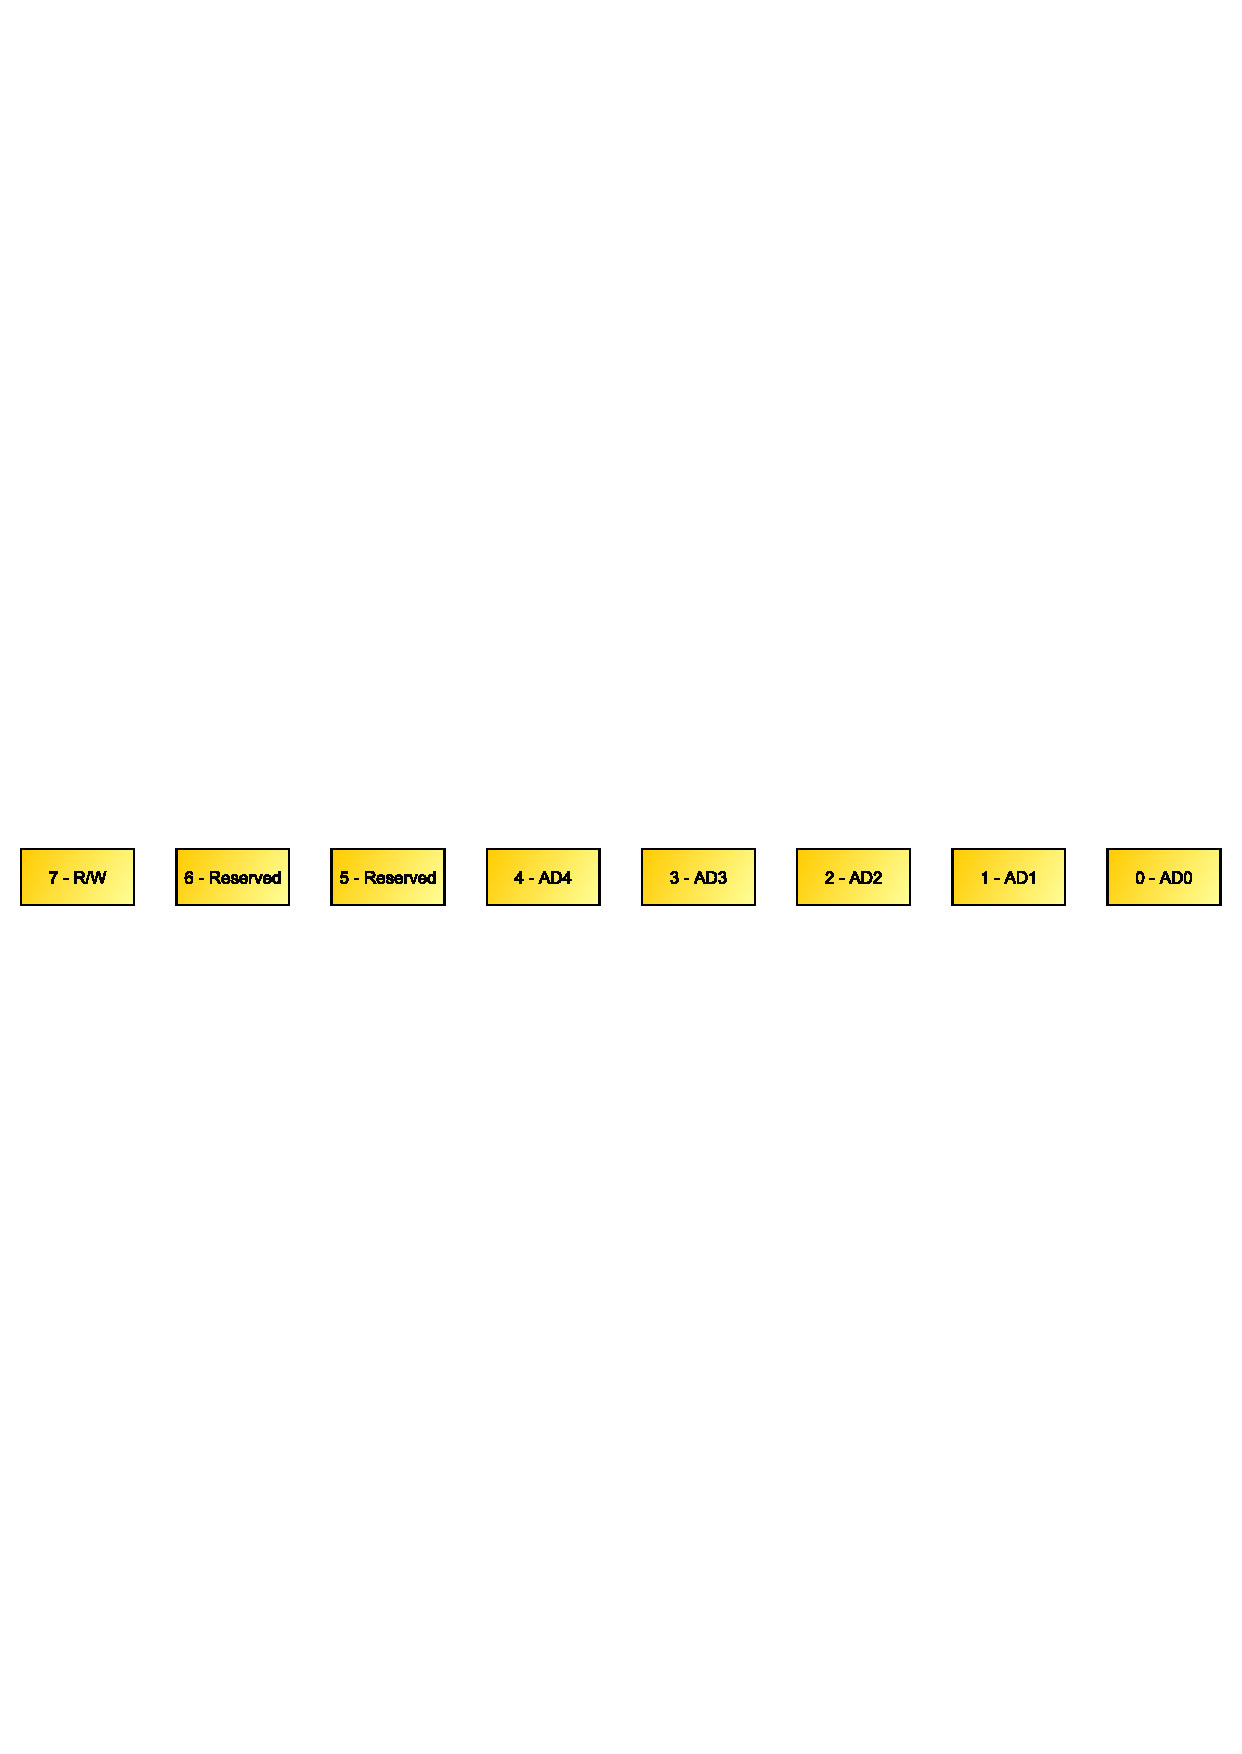
\includegraphics[scale=0.7,trim=0 390 0 390]{graphics/spi_protocol_cmd_structure.pdf} %trim=l b r t (can cut off from every side)
	\caption{Bit structure of the SPI command package send from master to slave}
	\label{fig:spi_protocol_cmd_structure}			% figure labels are of the form \label{fig:*}
	\end{center}
\end{figure}


\subsubsection{Reading from slave device}
When the master needs to read from the slave device it sends a byte with the MSB\footnote{Most significant bit} to low, and the last five bits according to the address to be read. Meanwhile the command is send, the slave may be sending the response from last command, or just zeroes if it has nothing to return. For the master to be able to receive the response, it needs to send a byte. This may be the next command or just zeroes. The reason for this is, that the communication is always initiated from the master device on SPI. A read command sequence is shown in figure \ref{fig:spi_protocol_command_structure_read} 

\begin{figure}[htb]
	\begin{center}
	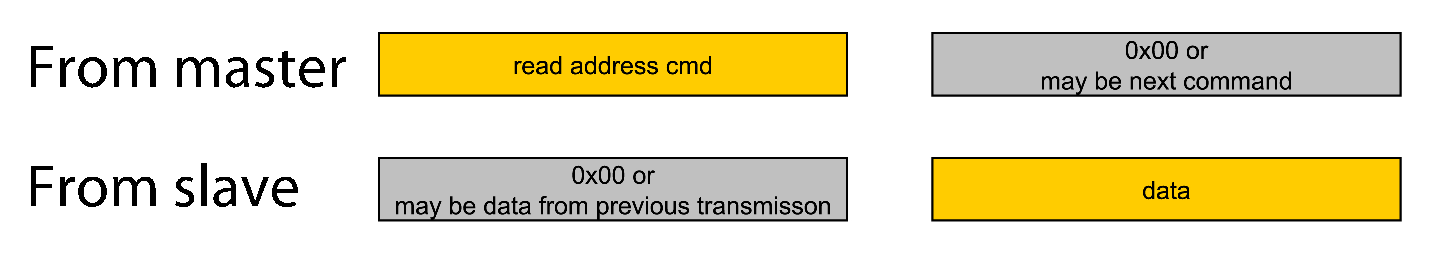
\includegraphics[scale=0.6,trim=0 0 0 0]{graphics/spi_protocol_command_structure_read_wlabels.pdf} %trim=l b r t (can cut off from every side)
	\caption{SPI communication when reading from the slave}
	\label{fig:spi_protocol_command_structure_read}			% figure labels are of the form \label{fig:*}
	\end{center}
\end{figure}


\subsubsection{Writing to slave device}
The command send from the master device when writing to the slave device is similar to the one used to read the same address, but with the MSB set to high. The structure of the command byte is shown in figure \ref{fig:spi_protocol_cmd_structure}. Meanwhile the command is send, the slave may be sending the response from last command, or just zeroes if it has nothing to return. Next the master sends the value to be written to the address from the command byte. While the value is send, the output from the slave is just an empty byte. The write sequence is shown in figure \ref{fig:spi_protocol_command_structure_write}.

\begin{figure}[htb]
	\begin{center}
	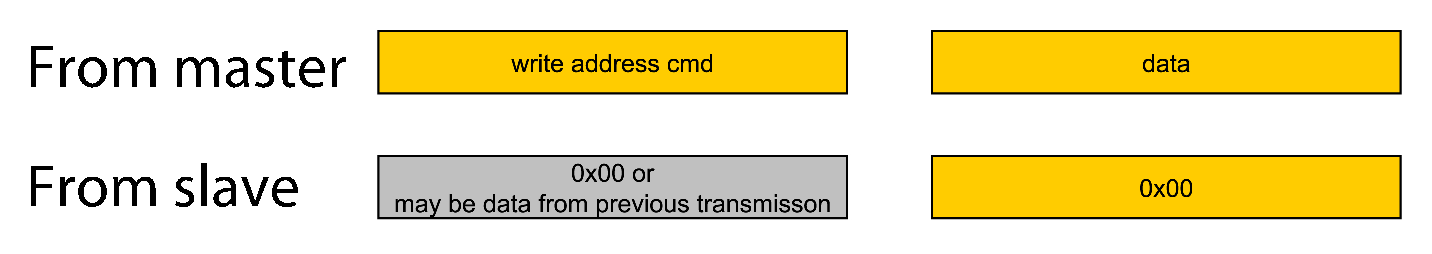
\includegraphics[scale=0.6,trim=0 0 0 0]{graphics/spi_protocol_command_structure_write_wlabels.pdf} %trim=l b r t (can cut off from every side)
	\caption{SPI communication when writing to the slave}
	\label{fig:spi_protocol_command_structure_write}			% figure labels are of the form \label{fig:*}
	\end{center}
\end{figure}



% Each frame is 9 bit. 8 bit data and escape bit. The escape bit is only high in the beginnign of each transmission.
% Freescale, because of the SSIFss high period to syncronize frames.

\subsection{Protocol ARM implementation}
\subsection{Protocol FPGA implementation}
The SPI client interface on the FPGA needs to written in hardware language. Before getting started writing the actual hardware description code, a block and signal description is made to clarify which parts that is needed, and how the internally communicate. Each block is then written in VHDL\footnote{Very high speed integrated circuit Hardware Description Language} and tested in a simulation test bench to ensure the correct functionality. The great advantage of a test bench is the possibility to quickly visualise both internal and external signals over time. When the hardware is tested to work in the simulation, it can be synthesized and put on the FPGA. On the FPGA it is tested with a AVR board with SPI interface, programmed with a code that is known to work. This will ensure that 

% Block overview / hardware planning
% Block description
% Testbench
